\chapter{Konzept}
\label{chap:konzept}
In diesem Kapitel wird das Konzept für die Entwicklung des ferngesteuerten Fahrzeugs beschrieben. Es werden die geplante Softwarearchitektur und der Hardwareaufbau erläutert. Zudem wird ein Vergleich verschiedener Video-Encoding-Methoden durchgeführt, um die beste Lösung für die Videoübertragung zu finden.

\section{Anforderungen}
In diesem Abschnitt werden die Anforderungen an das ferngesteuerte Fahrzeug beschrieben. Dazu gehören sowohl funktionale als auch nicht-funktionale Anforderungen, die für die Entwicklung des Fahrzeugs berücksichtigt werden müssen.

\subsection{Funktionale Anforderungen}
Das Fahrzeug soll in der Lage sein, über eine Weboberfläche gesteuert zu werden, um die Bewegungsrichtung und Geschwindigkeit zu regulieren. Zudem soll es Sensordaten und Kamerabilder in Echtzeit an die Weboberfläche übertragen können, um dem Benutzer die benötigten Informationen zur Steuerung des Fahrzeugs bereitzustellen.

\subsection{Nicht-funktionale Anforderungen}
Die Videoübertragung soll eine geringe Latenz aufweisen und eine mindest Framerate von 30 Bildern pro Sekunde erreichen, um eine flüssige Steuerung des Fahrzeugs zu ermöglichen. Die Kommunikation zwischen der Weboberfläche und dem Backend soll zuverlässig und stabil sein und eine möglichst geringe Latenz aufweisen, um eine praäzise und zufriedenstellende Steuerung zu ermöglichen.

\section{Hardwareaufbau}
    \subsection{Gehäuse}
    % anfangs 3d-gedruckt geplant, in umsetzung dann schreiben doch holz, weil stabiler, einfacher zu bearbeiten und leichter zu beschaffen/ersetzen 
    Zu Beginn des Projekts war geplant eine 3D-gedruckte Halterung zu verwenden, auf der alle Komponenten des Fahrzeugs montiert werden. Allerdings fiel die Entscheidung, stattdessen eine Halterung aus Holz zu verwenden. Dies liegt daran, dass Holz stabiler, einfacher zu bearbeiten und leichter zu beschaffen sowie zu ersetzen ist als 3D-gedrucktes Material. \\
    Insbesondere die einfache Bearbeitung ist ein entscheidender Punkt, da die Halterung voraussichtlich im Laufe des Projekts einige Male bearbeitet werden muss, um Anpassungen für die verschiedenen Komponenten vorzunehmen.

    Die Komponenten des Fahrzeugs werden so angeordnet, dass sie leicht zugänglich sind für Wartungsarbeiten und Anpassungen. Zudem wird darauf geachtet, dass das Gewicht der Komponenten gleichmäßig verteilt ist, um die Stabilität des Fahrzeugs zu gewährleisten.

    In Abbildung \ref{fig:gehaeuse} ist der Aufbau zu sehen, auf der alle Komponenten des Fahrzeugs montiert sind.
    \begin{figure}[H]
        \centering
        % \includegraphics[width=0.48\textwidth]{images/02Hardware/gehaeuse.png}
        %\vspace{-0.3cm}
        \caption{3D-gedruckte Halterung als Gehäuse}
        \vspace{-0.3cm}
        \label{fig:gehaeuse}
    \end{figure}

    \subsection{Komponenten}

        \subsubsection{Raspberry Pi}
        Als Steuergerät für das Fahrzeug wird ein Raspberry Pi verwendet. Der Raspberry Pi verfügt über ausreichend Leistung und Schnittstellen, um die Anforderungen des Projekts zu erfüllen. Ein Mikrocontroller wurde aufgrund der benötigten Rechenleistung und geplanten Features wie der Bildverarbeitung nicht in Betracht gezogen. \\
        Der Raspberry Pi ermöglicht die Ansteuerung der Motoren mit mithilfe der \ac{GPIO} Pins, die Verarbeitung der Sensordaten und die Kommunikation mit der Weboberfläche. Zudem bietet er die Möglichkeit, verschiedene Bibliotheken und Frameworks zu nutzen, um die Implementierung

        \subsubsection{Motoren}
        Die beiden Motoren werden direkt an die beiden Räder des Fahrzeugs montiert. Um das Fahrzeug zu bewegen, werden die Motoren jeweils in die gleiche Richtung bewegt. Das Lenken erfolgt durch die Ansteuerung der Motoren in unterschiedliche Richtungen. Wenn beispielsweise der linke Motor vorwärts und der rechte Motor rückwärts angetrieben wird, dreht sich das Fahrzeug nach rechts und umgekehrt. Durch die Möglichkeit, die Motoren unabhängig voneinander zu steuern, kann das Fahrzeug präzise manövriert werden, was insbesondere bei der Umsetzung von Fahrassistenzsystemen von Vorteil ist.

        Die Motoren verfügen über eine interne Getriebeübersetzung, welche die Drehzahl reduziert und das Drehmoment erhöht. Dies ermöglicht eine präzisere Steuerung des Fahrzeugs und im Vergleich zu einem Motor ohne Getriebe ein höheres Drehmoment, was insbesondere bei niedrigen Geschwindigkeiten von Vorteil ist. 

        \subsection{Akku}
        Zur Stromversorgung des Fahrzeugs wird ein \ac{LiPo} Akku verwendet. Aufgrund der hohen Energiedichte ist ein \ac{LiPo} Akku eine solide Wahl für den Anwendungszweck. Jedoch gibt es auch einige Nachteile. Die Zellchemie des Akkus ist sehr empfindlich gegenüber Tiefenentladung sowie mechanischen Beschädigungen, weshalb eine sorgfältige Handhabung und Überwachung der Akkus notwendig ist. 

        Eine Alternative Zell-Chemie wäre beispielsweise ein \ac{LiFePO} Akku, welcher eine höhere Sicherheit bietet, jedoch eine geringere Energiedichte aufweist. Da das geplante Gehäuse nur begrenzten PLatz für den Akku bietet, wurde die Entscheidung getroffen, einen \ac{LiPo} Akku zu verwenden, um eine ausreichende Kapazität zu gewährleisten.

        \subsection{Hall-Sensor}
        Zur Messung der Geschwindigkeit des Fahrzeugs wird ein Hall-Sensor verwendet. Dieser erkennt die Anwesenheit eines magnetischen Feldes, welches von einem Magneten erzeugt wird, der an einem der Räder befestigt ist. Durch die Erkennung der Umdrehungen des Rades kann die Geschwindigkeit des Fahrzeugs berechnet werden. 

        Auf die Verwendung von Encodern wurde bewusst verzichtet, da diese in der Regel teurer und komplexer in der Ansteuerung sind als Hall-Sensoren. Zudem bieten Hall-Sensoren eine ausreichende Genauigkeit für die geplanten Fahrassistenzsysteme, weshalb die Entscheidung getroffen wurde, einen Hall-Sensor zu verwenden.

        \subsection{Spannungswandler}
        Da die Motoren eine Nennspannung von 6 Volt und der Raspberry Pi eine Nennspannung von 5 Volt haben, werden mehrere Spannungsregler verwendet, um die benötigten Spannungen für die verschiedenen Komponenten bereitzustellen. Ein Abwärtswandler wird verwendet, um die Spannung von 7,4 Volt auf 5 Volt zu reduzieren, um den Raspberry Pi mit Strom zu versorgen. Zwei weitere Step-Down Spannungsregler werden verwendet, um die Spannung von 7,4 Volt auf 6 Volt zu reduzieren, um die Motoren mit Strom zu versorgen.

        Ein einzelner Spannungswandler kann nur maximal 5 Ampere ausgeben. Da der Raspberry Pi unter Volllast alleine bereits 5 Ampere aufnehmen kann, ist es notwendig, mehrere Spannungswandler zu verwenden, um die benötigten Spannungen für die verschiedenen Komponenten bereitstellen zu können.

% motoren
\section{Softwarearchitektur}

     \begin{figure}[H]
        \centering
         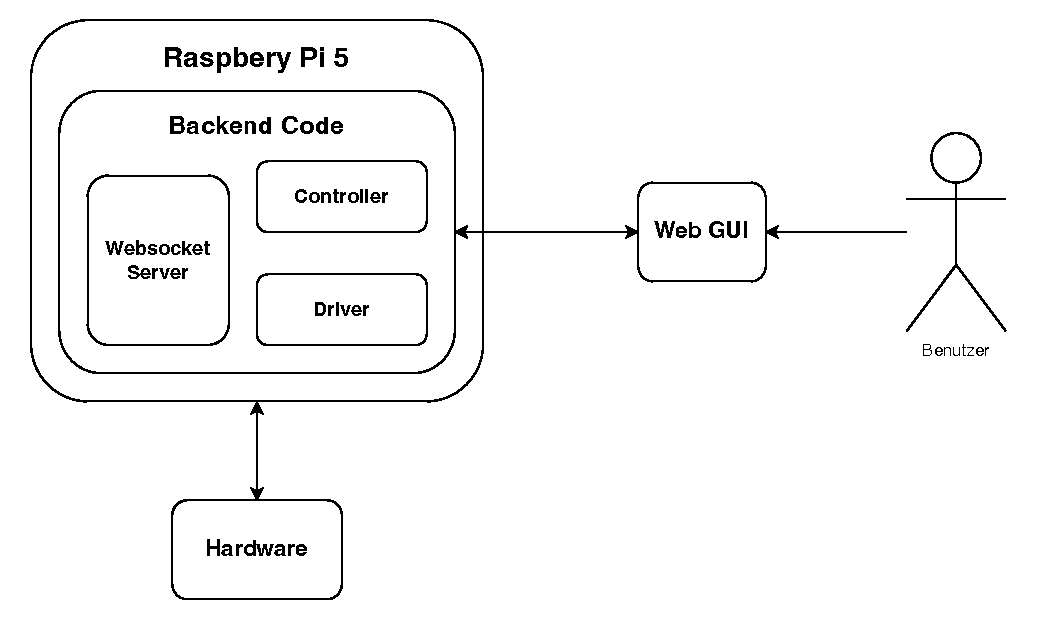
\includegraphics[width=0.7\textwidth]{images/04Konzept/software_overview.drawio.pdf}
        \vspace{-0.3cm}
        \caption{Übersicht }
        \vspace{-0.3cm}
        \label{fig:software_overview}
    \end{figure}


    \subsection{Weboberfläche zur Steuerung und Überwachung}
    Dem User wird eine Weboberfläche zur Verfügung über die das Fahrzeug gesteuert und überwacht werden kann. Hierzu werden Sensordaten und Kamerabilder in Echtzeit vom Fahrzeug an die Weboberfläche übertragen, um dem Benutzer die benötigten Informationen zur Steuerung des Fahrzeugs bereitzustellen. Über die Weboberfläche können zudem Steuerbefehle an das Fahrzeug gesendet werden, um beispielsweise die Geschwindigkeit zu regulieren oder die Richtung zu ändern.

    \subsection{Backend-Anwendung zur Ansteuerung der Hardware}
    Das Backend ist für die direkte Ansteuerung der Hardwarekomponenten des Fahrzeugs zuständig. Es empfängt die Steuerbefehle von der Weboberfläche und wertet diese aus, um die entsprechenden Vorgänge und Aktionen durchzuführen. Dazu gehört beispielsweise die Ansteuerung der Motoren bei Regulierung der Geschwindigkeit. \\
    Zudem verarbeitet das Backend die Sensordaten und Kamerabilder, um die geplanten Fahrassistenzsysteme wie die Notbremsung oder Follow the line zu implementieren. Diese werden ohne direkte Interaktion des Benutzers automatisch ausgelöst, wenn die entsprechenden Bedingungen erfüllt sind, weshalb diese vollständig im Backend verarbeitet werden.

    \subsection{Kommunikation zwischen GUI und Backend}
    Für die Kommunikation zwischen der GUI-Anwendung und der Backend-Anwendung wird ein Websocket verwendet. Ein Websocket ermöglicht eine bidirektionale Kommunikation zwischen einem Server und mehreren Clients. In diesem Projekt nimmt der Raspberry Pi die Rolle des Servers ein, während die Weboberfläche als Client fungiert. 

    \subsection{Video-Encoding Vergleich}
    % Tabelle mit Vor- und Nachteilen der verschiedenen Methoden, sowie die geplante Methode und Begründung für die Wahl

    \subsection{Implementierte Features} % vielleicht vor Softwarekomponenten? Weil da werden schon Features erwähnt
    In diesem Abschnitt werden die für das Fahrzeug geplanten Features beschrieben.

    \subsubsection{Notbremsung durch Hinderniserkennung}
    Das Fahrzeug soll in der Lage sein, eine Notbremsung durchzuführen, wenn es ein Hindernis erkennt. Hierzu werden Ultraschallsensoren verwendet, die den Bereich vor dem Fahrzeug überwachen und die Entfernung zu Hindernissen messen. Wird ein Hindernis erkannt, das eine Kollision verursachen könnte, wird automatisch eine Notbremsung eingeleitet. Um zu ermitteln, ob eine Kollision wahrscheinlich ist, wird die gemessene Entfernung unter Berücksichtigung der aktuellen Geschwindigkeit des Fahrzeugs ausgewertet. 

    \subsubsection{Schilderkennung}

    \subsubsection{Fernsteuerung}
    
    \subsubsection{Follow the line}
    \subsubsection{etc.}


% Hardware-Aufbau:
%     Komponentenübersicht:
%         - Auflistung der verwendeten Hardware (z. B. Sensoren, Aktoren, Mikrocontroller, Stromversorgung).
%     Systemarchitektur:
%         - Blockdiagramm oder Beschreibung der Verbindungen zwischen den Komponenten.
%     Materialwahl:
%         - Begründung der Auswahl (z. B. Holz vs. 3D-Druck, spezifische Bauteile).
%     Mechanische Konstruktion:
%         - Aufbau des Gehäuses oder Rahmens.
%         - Befestigung der Komponenten.
%     Energieversorgung:
%         - Stromquelle (z. B. Batterie, Netzteil).
%         - Energiebedarf und Effizienz.
%     Kommunikation:
%         - Schnittstellen (z. B. I2C, SPI, UART, CAN-Bus).
%     Erweiterbarkeit:
%         - Möglichkeit, zusätzliche Module oder Funktionen hinzuzufügen.

% Software-Aufbau:
%     Systemübersicht:
%         - Beschreibung der Softwarearchitektur (z. B. Schichtenmodell, Module).
%     Programmiersprache und Frameworks:
%         - Begründung der Wahl (z. B. Python, C++, ROS).
%     Hauptfunktionen:
%         - Steuerung der Hardware.
%         - Datenverarbeitung (z. B. von Sensoren).
%     Benutzerinteraktion (z. B. GUI, Webinterface).
%     Kommunikation:
%         - Protokolle (z. B. MQTT, HTTP, WebSocket).
%         - Datenformate (z. B. JSON, XML).
%     Fehlerbehandlung:
%         - Strategien zur Erkennung und Behandlung von Fehlern.
%     Modularität:
%         - Möglichkeit, Funktionen zu erweitern oder zu ändern.
%     Testbarkeit:
%         - Unit-Tests, Integrationstests.
%     Sicherheitsaspekte:
%         - Schutz vor unbefugtem Zugriff.
%         - Datenintegrität.
%     Allgemein:
%         - Zusammenspiel von Hardware und Software:
%             - Wie die Software die Hardware steuert.
%             - Datenfluss zwischen den Komponenten.
%     Ziele und Anforderungen:
%         - Funktionale Anforderungen (z. B. Leistung, Genauigkeit).
%         - Nicht-funktionale Anforderungen (z. B. Robustheit, Skalierbarkeit).
%     Zeitplan und Meilensteine:
%         - Wichtige Schritte bei der Umsetzung.